\documentclass[a4paper, 12pt]{article}
\usepackage[utf8]{inputenc}

\usepackage[top=.25in,bottom=.25in,left=.25in,right=.25in]{geometry}
\usepackage[parfill]{parskip}
\usepackage{courier}
\usepackage{graphicx}

\usepackage{listings}
\lstset{
    frame=single,
    breaklines=true,
    basicstyle=\footnotesize\ttfamily
}

\begin{document}
\pagenumbering{gobble}

\begin{figure}[h!]
    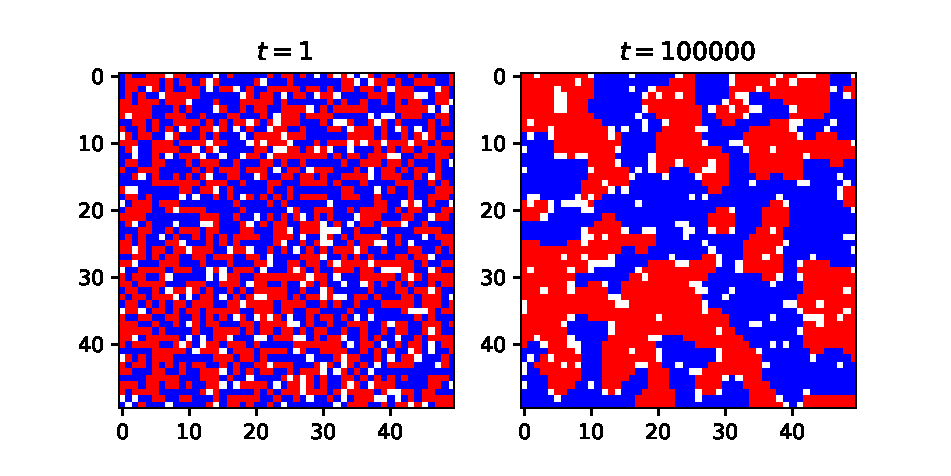
\includegraphics[width=\linewidth]{../Schelling-Model/town.pdf}
\end{figure}

\begin{figure}[h!]
    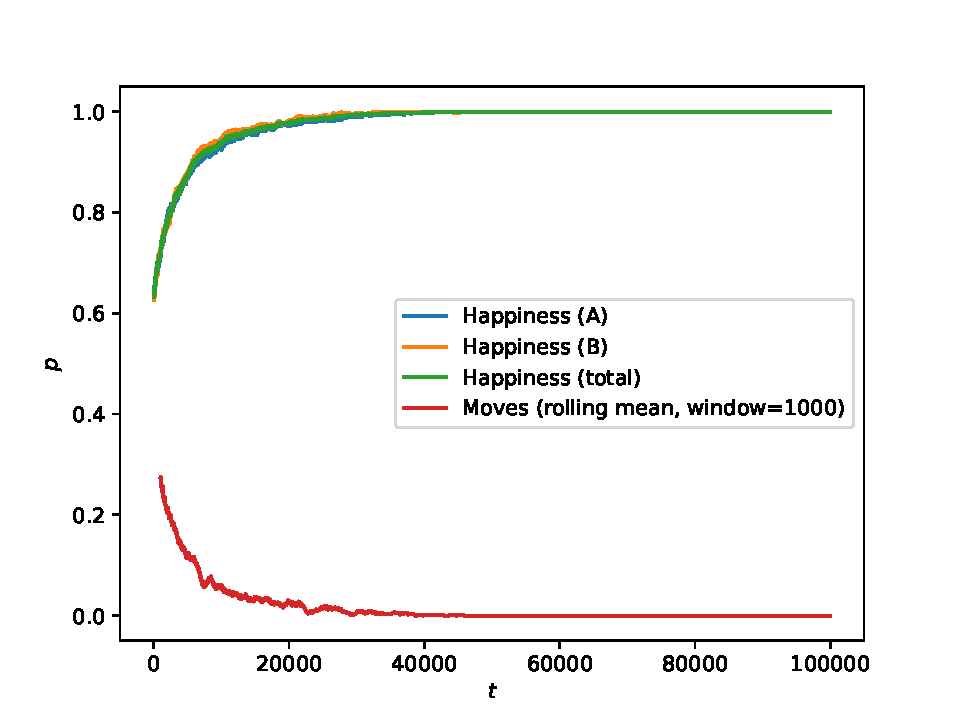
\includegraphics[width=\linewidth]{../Schelling-Model/happiness.pdf}
\end{figure}

\newpage

\begin{figure}[h!]
    \centering
    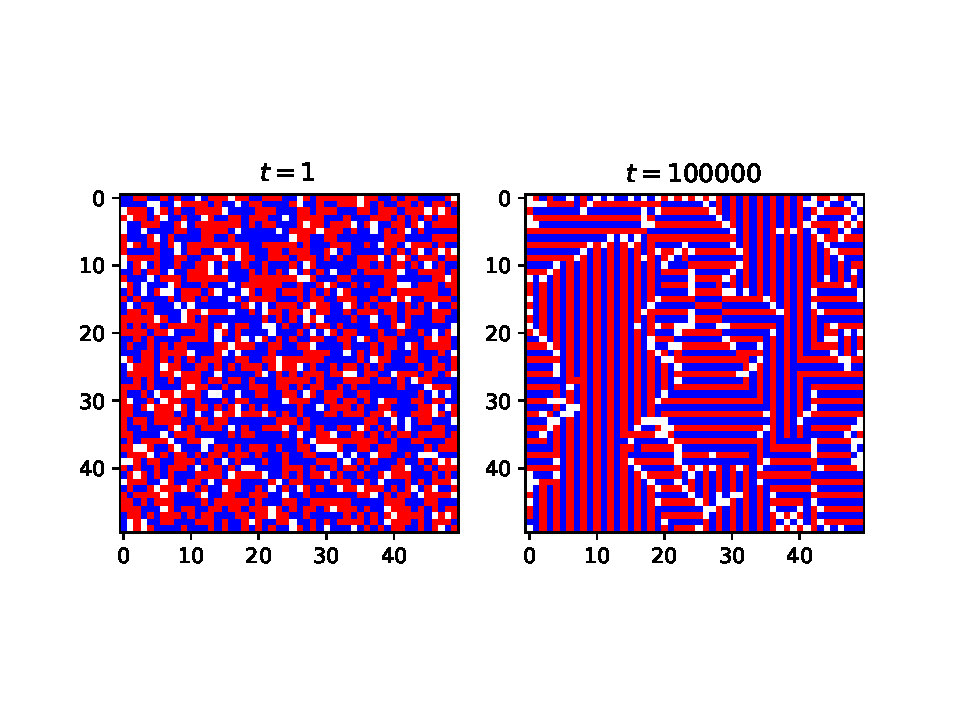
\includegraphics[width=0.9\linewidth]{../Anti-Gregarious/town.pdf}
\end{figure}

\begin{figure}[h!]
    \centering
    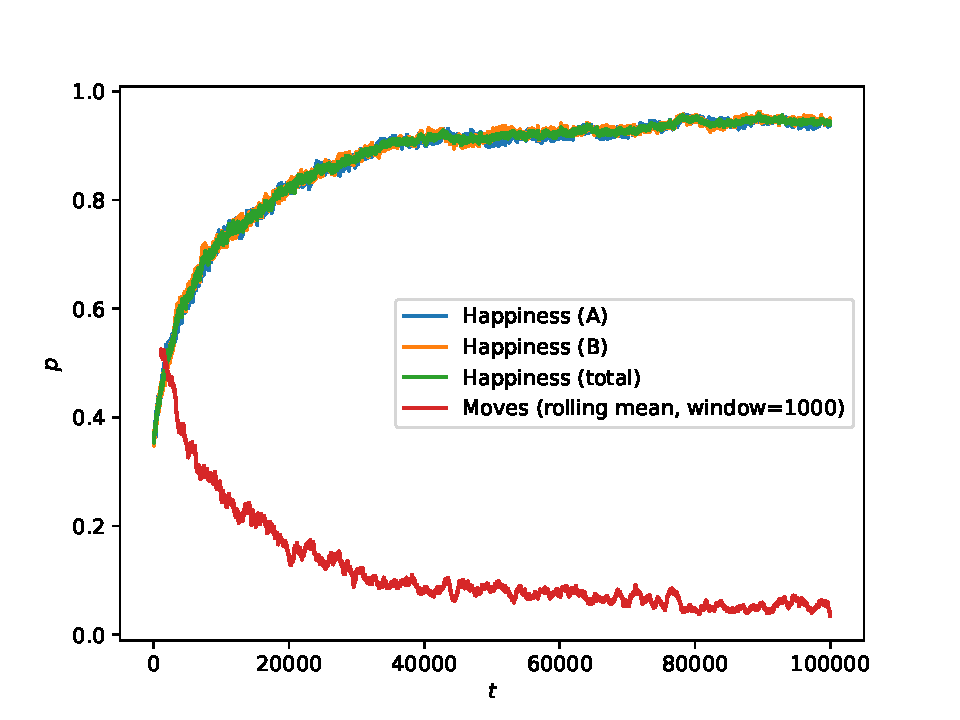
\includegraphics[width=0.9\linewidth]{../Anti-Gregarious/happiness.pdf}
\end{figure}

\newpage

\begin{figure}[h!]
    \centering
    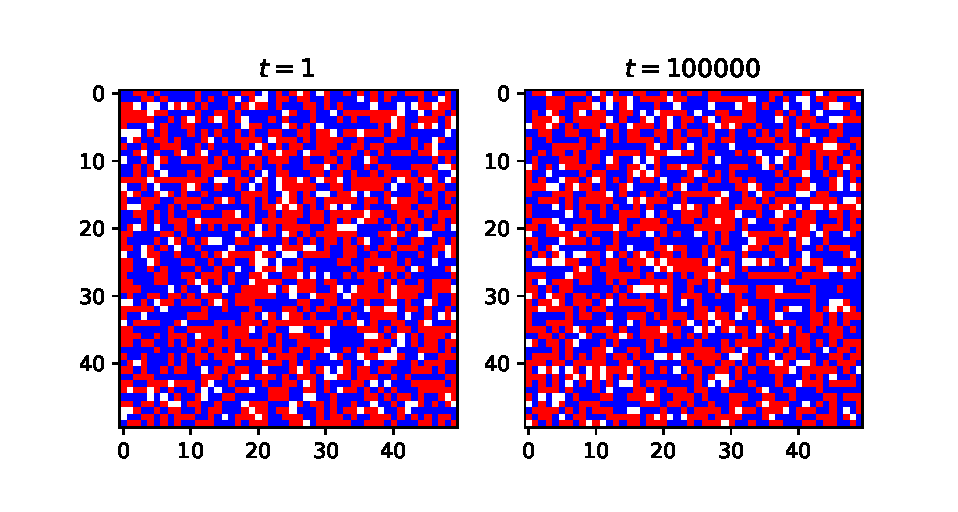
\includegraphics[width=\linewidth]{../Frustration/town.pdf}
\end{figure}

\begin{figure}[h!]
    \centering
    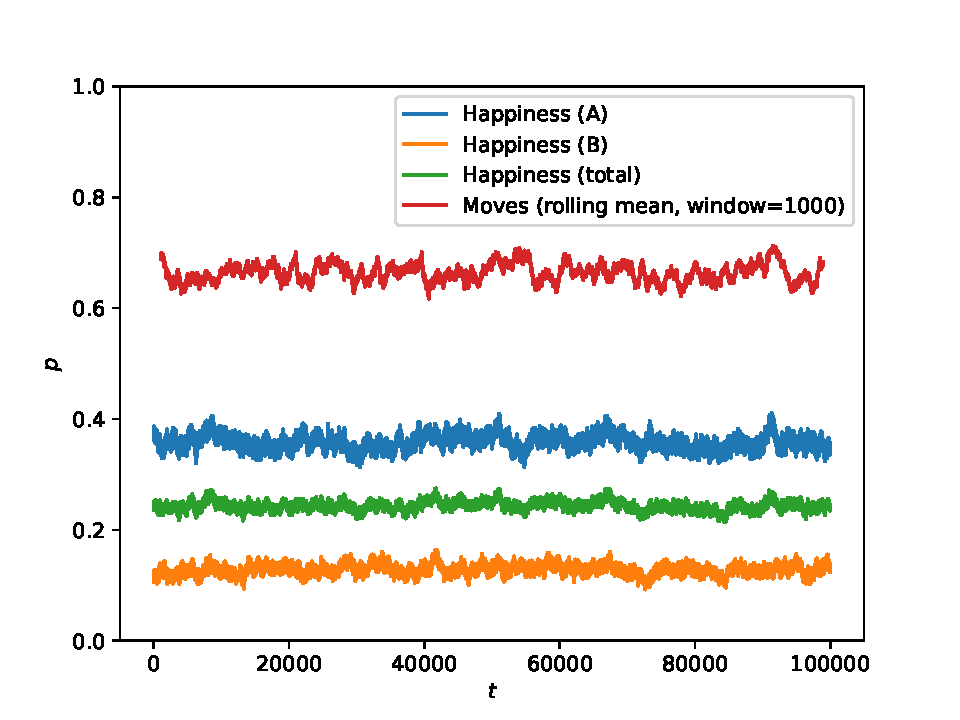
\includegraphics[width=\linewidth]{../Frustration/happiness.pdf}
\end{figure}

\newpage

\begin{figure}[h!]
    \centering
    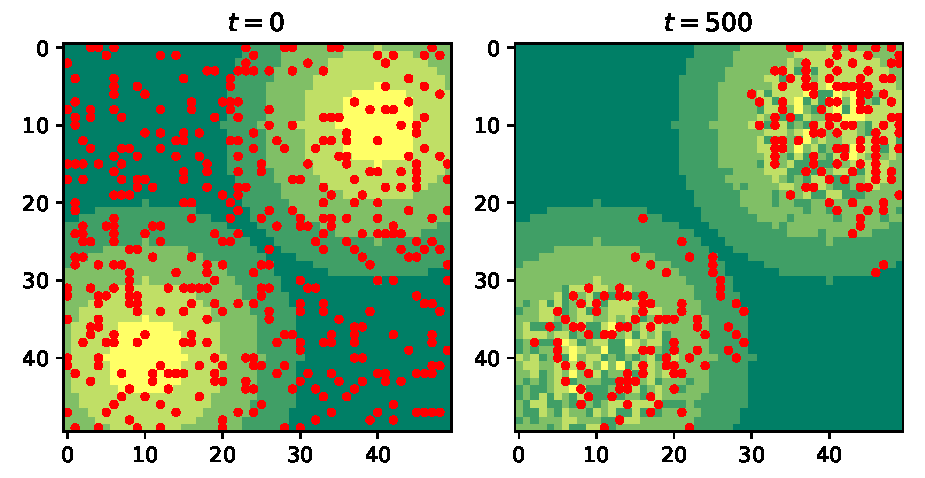
\includegraphics[width=0.8\linewidth]{../Sugar-Scape/c.pdf}
\end{figure}

\begin{figure}[h!]
    \centering
    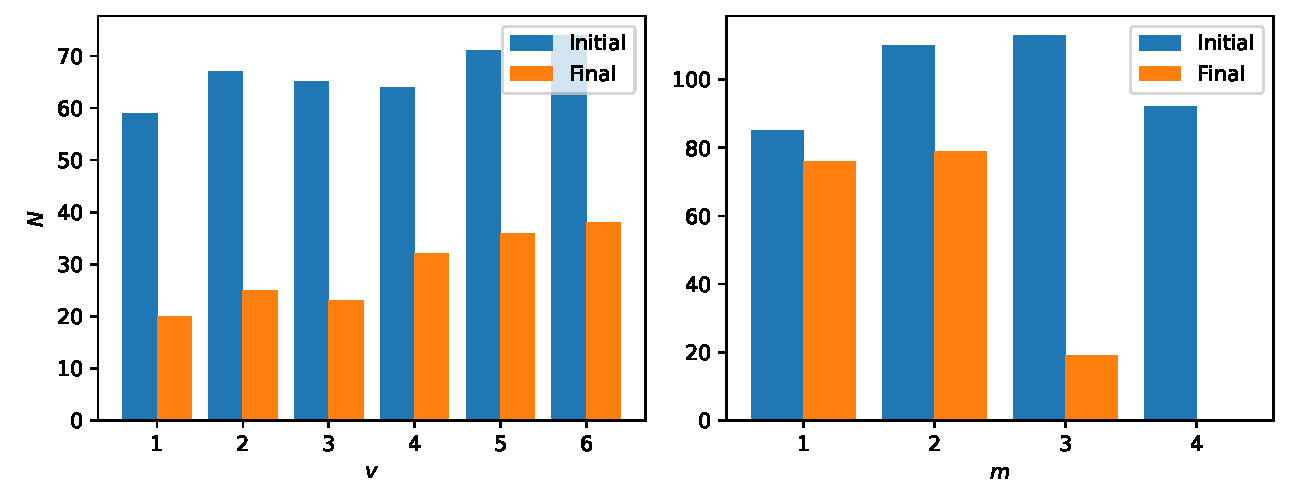
\includegraphics[width=\linewidth]{../Sugar-Scape/d.pdf}
\end{figure}

\begin{figure}[h!]
    \centering
    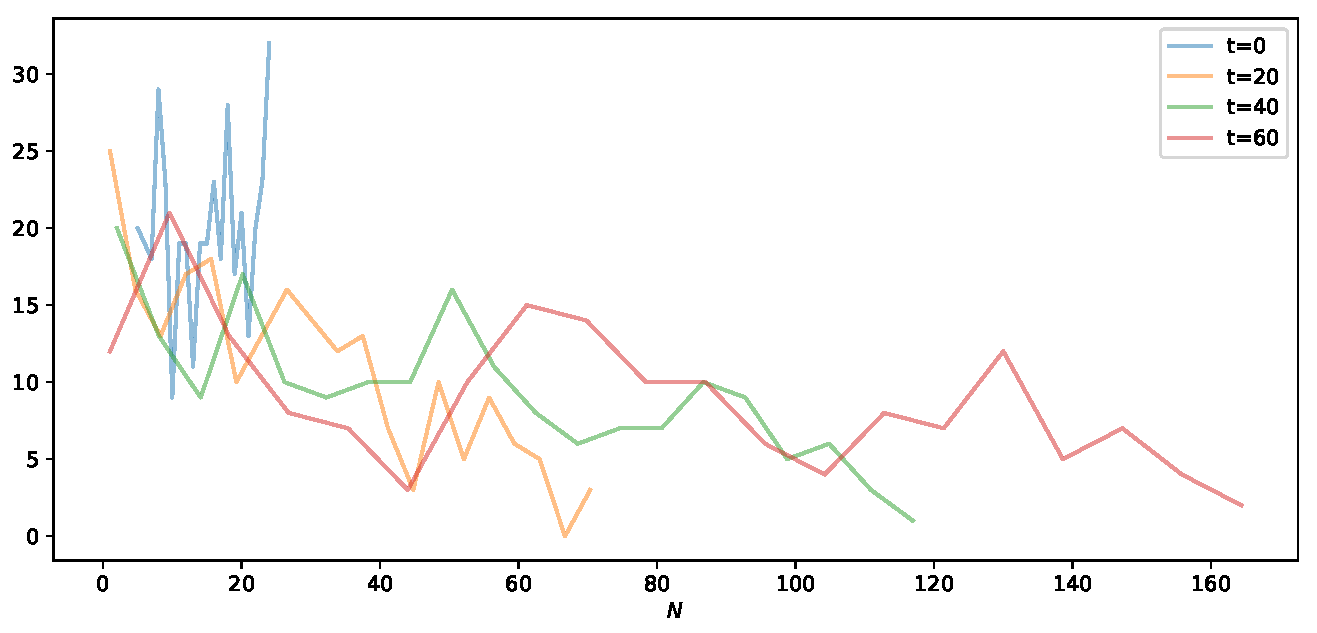
\includegraphics[width=\linewidth]{../Sugar-Scape/e.pdf}
\end{figure}


\newpage

/Schelling-Model/main.py
\lstinputlisting{../Schelling-Model/main.py}
\newpage

/Anti-Gregarious/main.py
\lstinputlisting{../Anti-Gregarious/main.py}
\newpage

/Frustration/main.py
\lstinputlisting{../Frustration/main.py}
\newpage

/Sugar-Scape/main.py
\lstinputlisting{../Sugar-Scape/main.py}
\newpage

\end{document}
